\documentclass[tikz,border=6pt]{standalone}
\usepackage[T1]{fontenc}
\usepackage{lmodern}
\usepackage{amsmath}
\usepackage{pgfplots}
\pgfplotsset{compat=1.18}
\usetikzlibrary{arrows.meta,positioning,fit,backgrounds,shapes.geometric,calc}
\definecolor{navy}{HTML}{16324F}
\definecolor{tealC}{HTML}{007F82}
\definecolor{amberC}{HTML}{D97706}
\definecolor{coralC}{HTML}{C2410C}
\definecolor{redC}{HTML}{DC2626}
\definecolor{mintC}{HTML}{059669}
\definecolor{slateC}{HTML}{64748B}
\definecolor{paleBg}{HTML}{F4F7FA}
\definecolor{softTeal}{HTML}{E6F4F4}
\definecolor{softNavy}{HTML}{EAF0F6}
\definecolor{softAmber}{HTML}{FEF3C7}
\begin{document}

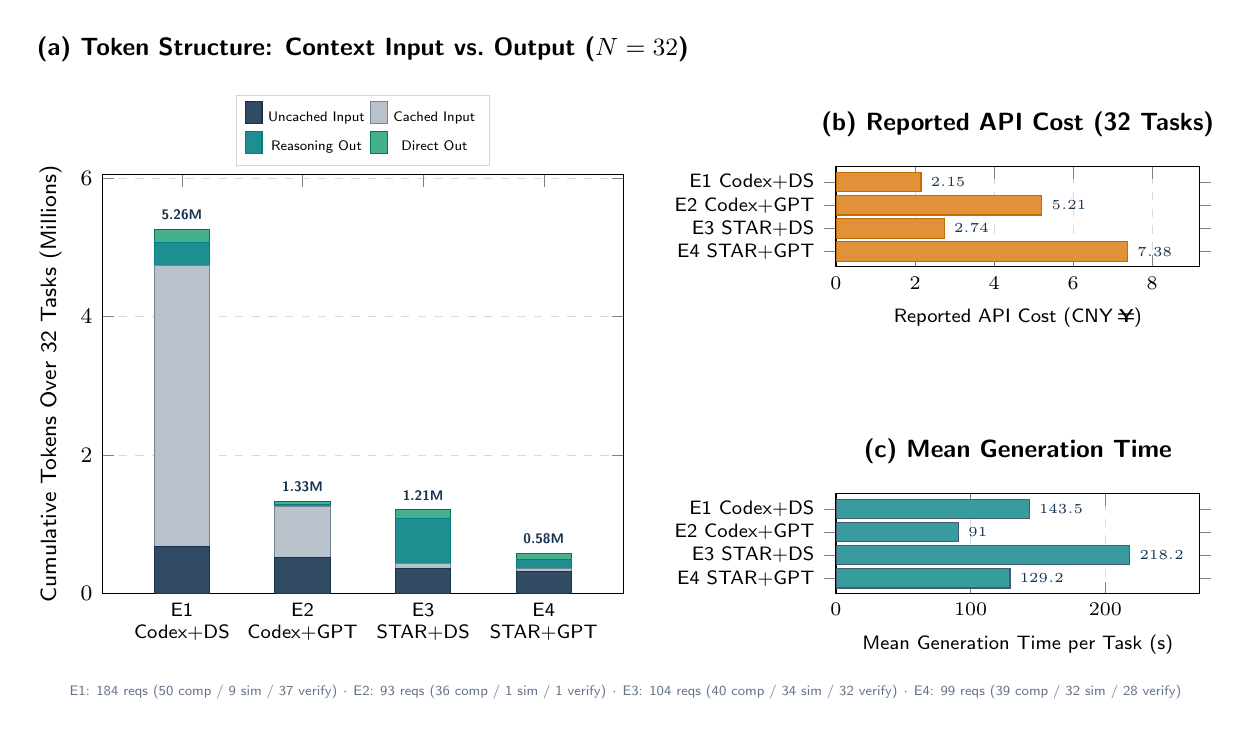
\begin{tikzpicture}
\begin{axis}[
    name=leftax,
    ybar stacked,
    bar width=20pt,
    width=8.2cm,
    height=6.9cm,
    ymin=0, ymax=6.05,
    ylabel={\footnotesize Cumulative Tokens Over 32 Tasks (Millions)},
    xtick={0,1,2,3},
    xticklabels={E1\\Codex+DS, E2\\Codex+GPT, E3\\STAR+DS, E4\\STAR+GPT},
    x tick label style={font=\scriptsize\sffamily, align=center},
    tick label style={font=\footnotesize\sffamily},
    label style={font=\footnotesize\sffamily},
    title={\small\sffamily\bfseries (a) Token Structure: Context Input vs.\ Output ($N=32$)},
    title style={yshift=11mm},
    legend style={at={(0.5,1.02)}, anchor=south, legend columns=2, font=\tiny\sffamily, draw=navy!20, fill=white},
    ymajorgrids=true,
    grid style={dashed, gray!30},
    enlarge x limits=0.22,
]
\addplot[fill=navy!88, draw=navy] coordinates {(0,0.685) (1,0.519) (2,0.358) (3,0.324)};
\addplot[fill=navy!30, draw=navy!60] coordinates {(0,4.057) (1,0.742) (2,0.075) (3,0.041)};
\addplot[fill=tealC!88, draw=tealC] coordinates {(0,0.331) (1,0.021) (2,0.651) (3,0.126)};
\addplot[fill=mintC!75, draw=mintC!80!black] coordinates {(0,0.184) (1,0.052) (2,0.127) (3,0.09)};
\legend{Uncached Input, Cached Input, Reasoning Out, Direct Out}
\node[font=\tiny\sffamily\bfseries, color=navy, anchor=south] at (axis cs:0,5.26) {5.26M};
\node[font=\tiny\sffamily\bfseries, color=navy, anchor=south] at (axis cs:1,1.33) {1.33M};
\node[font=\tiny\sffamily\bfseries, color=navy, anchor=south] at (axis cs:2,1.21) {1.21M};
\node[font=\tiny\sffamily\bfseries, color=navy, anchor=south] at (axis cs:3,0.58) {0.58M};
\end{axis}

\begin{axis}[
    name=topr,
    at={($(leftax.north east)+(27mm,1mm)$)},
    anchor=north west,
    xbar,
    bar width=7pt,
    width=6.2cm,
    height=2.85cm,
    xmin=0, xmax=9.2,
    xlabel={\scriptsize Reported API Cost (CNY \textyen)},
    ytick={0,1,2,3},
    yticklabels={E4 STAR+GPT, E3 STAR+DS, E2 Codex+GPT, E1 Codex+DS},
    tick label style={font=\scriptsize\sffamily},
    label style={font=\scriptsize\sffamily},
    title={\small\sffamily\bfseries (b) Reported API Cost (32 Tasks)},
    title style={yshift=0.5mm},
    xmajorgrids=true,
    grid style={dashed, gray!30},
    nodes near coords,
    every node near coord/.append style={font=\tiny\sffamily\bfseries, color=navy, anchor=west},
    enlarge y limits=0.22,
]
\addplot[fill=amberC!80, draw=amberC!90!black] coordinates {(2.15,3) (5.21,2) (2.74,1) (7.38,0)};
\end{axis}

\begin{axis}[
    name=botr,
    at={($(leftax.south east)+(27mm,0mm)$)},
    anchor=south west,
    xbar,
    bar width=7pt,
    width=6.2cm,
    height=2.85cm,
    xmin=0, xmax=270,
    xlabel={\scriptsize Mean Generation Time per Task (s)},
    ytick={0,1,2,3},
    yticklabels={E4 STAR+GPT, E3 STAR+DS, E2 Codex+GPT, E1 Codex+DS},
    tick label style={font=\scriptsize\sffamily},
    label style={font=\scriptsize\sffamily},
    title={\small\sffamily\bfseries (c) Mean Generation Time},
    title style={yshift=0.5mm},
    xmajorgrids=true,
    grid style={dashed, gray!30},
    nodes near coords,
    every node near coord/.append style={font=\tiny\sffamily\bfseries, color=navy, anchor=west},
    enlarge y limits=0.22,
]
\addplot[fill=tealC!78, draw=navy!80] coordinates {(143.5,3) (91.0,2) (218.2,1) (129.2,0)};
\end{axis}

\node[font=\tiny\sffamily, color=slateC, anchor=north, align=center] at ($(current bounding box.south)+(0,-1.5mm)$)
  {E1: 184 reqs (50 comp / 9 sim / 37 verify) $\cdot$ E2: 93 reqs (36 comp / 1 sim / 1 verify) $\cdot$ E3: 104 reqs (40 comp / 34 sim / 32 verify) $\cdot$ E4: 99 reqs (39 comp / 32 sim / 28 verify)};
\end{tikzpicture}
\end{document}
